\documentclass{article} % For LaTeX2e
\usepackage{nips13submit_e,times}
\usepackage{hyperref}
\usepackage{url}
\usepackage{tikz,amsmath}
%\documentstyle[nips13submit_09,times,art10]{article} % For LaTeX 2.09


\title{Project Report: Digit Recognizer}

\author{
Jimmy Lin (xl5224) \\
Department of Computer Science\\
University of Texas at Austin\\
Austin, TX 78712 \\
\texttt{JimmyLin@utexas.edu} \\
%{{{ For More Author
\And
Jisong Yang (jy7226) \\
Department of Statistical Scientfic Computation\\
University of Texas at Austin\\
Austin, TX 78712 \\
\texttt{jsyang993@gmail.com} \\
%\AND
%Coauthor \\
%Affiliation \\
%Address \\
%\texttt{email} \\
%\And
%Coauthor \\
%Affiliation \\
%Address \\
%\texttt{email} \\
%\And
%Coauthor \\
%Affiliation \\
%Address \\
%\texttt{email} \\
%(if needed)\\
%}}}
}

% The \author macro works with any number of authors. There are two commands
% used to separate the names and addresses of multiple authors: \And and \AND.
%
% Using \And between authors leaves it to \LaTeX{} to determine where to break
% the lines. Using \AND forces a linebreak at that point. So, if \LaTeX{}
% puts 3 of 4 authors names on the first line, and the last on the second
% line, try using \AND instead of \And before the third author name.

\newcommand{\fix}{\marginpar{FIX}}
\newcommand{\new}{\marginpar{NEW}}

\nipsfinalcopy % Uncomment for camera-ready version


% TODO: Find a report guideline 
% TODO: 
\begin{document}


\maketitle

\begin{abstract}
    BACKGROUND. The idea of recognizing digit . 
    The goal in this project is to take an image of a handwritten single
    digit, and determine what that digit is.  
    
    Kaggle competition. 
    We propose to 

\end{abstract}

\section{Introduction}
% MOTIVATION SENTENCE
Recognizing hand-written characters has long been a hot topic in artificial
intelligence community. 
% KEY CONCEPT (PROBLEM) ILLUMINATION
Handwriting recognition is the ability of a computer to receive and
interpret intelligible handwritten input from sources such as paper documents,
photographs, touch-screens and other devices.
% SUMMARIZE THE SOLUTION
In the past decades, many probabilistic or non-probabilistic algorithms have
been exploited to effectively solve this problem, including K-nearest
neighbour, random forest, and well-known neural network. 

% ORGANIZATION OF THIS REPORT
In this report, we will illuminate the motivation of digit recognition
problem on section \ref{Motivation}. In section \ref{Details}, the
 main algorithms exploited in this project will be present to reader. For each
 algorithm, the algorithmic introduction, the reason of attempting that
 algorithm and finally corresponding implementation details will be indicated. 

\section{Motivations} \label{Motivation}
% APPLICATION OF THIS PROBLEM 
As to the historical application of handwriting recognition, 
it can be traced back to early 1980s.  There are plenty of commercial products
incorporating handwriting recognition as a replacement for keyboard input were
introduced. The hardware application continued to develop
in the following decades.  Until the recent years, Tablet PCs can be regarded
as a special notebook computer that is outfitted with a digitizer tablet and a
stylus, and allows a user to handwrite text on the unit's screen. In addition,
highly efficient handwriting recognizers were developed in real world to apply
on the zip codes detection.

\begin{figure}[h]
    \centering
    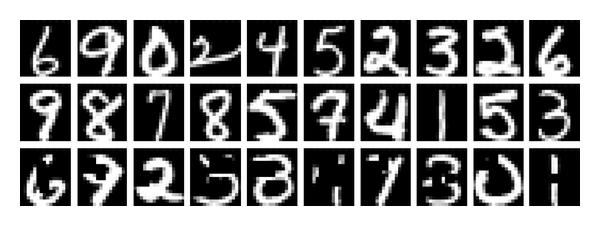
\includegraphics[width=3.5in,height=1.5in]{./857453.jpg}\\
    \caption{Digit Recognition Examples}
\end{figure}

% RELATED WORKS/SOLUTION
Plenty of mature solutions has already been developed to existence in solving
the handwriting problem. 
Since 2009, the recurrent neural networks and deep feedforward neural networks
developed in the research group of Jürgen Schmidhuber at the Swiss AI Lab
IDSIA have outshined many other models in competitions.
% POSSIBLE IMPROVEMENTS?
The fact that existing algorithms are powerful in recognizing digits does not
remove possibility of further improvement. The chance of improvement lies in
reduction of computational complexity for recognizing digits in higher degree.

\section{Implementation Details} \label{Details}
\subsection{Data Preprocessing} 
% INTRODUCITON OF PCA
{\bf Principal Component Analysis} (PCA) is a statistical procedure that uses
orthogonal transformation to convert a set of observations of possibly
correlated variables into a set of values of linearly uncorrelated variables
called principal components. Typically, the number of principal components is
no more than the number of original variables. That is to say, a particular
subspace, whose bases are independent to each other, is generated by such
tranformation. This transformation is defined in such a way that the first
principal component has the largest possible variance, and each succeeding
component in turn has the highest variance possible under the constraint that
it is orthogonal to the preceding components. In section \ref{Comparison}, the
performance comparisons of different algorithms will be illustrated and after
which, we will make conclusion about which one achieve the best performance. 

% why use PCA
In our project, we make use of PCA as dimensionality reduction for preprocessing the raw input image data.
Since the raw data explictly characterize the gray value of each pixels, each
handwritten instance is extremely high-dimensional. Although directly using
the raw input data avoids loss of information, the computational complexity
would be unresonably large. Put it another way, we have to think of a way to
compromise the ultimate accuracy to achieve a less computational cost on that
algorithm.

% implementation detail
However, several details matter significantly to the effect of PCA. One is the number
of principal components employed. If too many principal components are used,
it is far from reaching the goal of dimensionality reduction. However, we may
lose useful information for latter prediction if important components are not
used. Note that even least useful principal components contain disjoint information
that may contribute to latter prediction performance. As to our
implementation, we choose to pick up the set of principal components whose
eigenvalues are significantly greater than the others. 

{\large [TODO: How many components do we use in total?]}

% reference

\subsection{Neural Network}
% INTRODUCTION TO NEURAL NETWORK
In the field of machine learning, {\bf neural networks} are computational models
inspired by animals' central nervous systems (in particular the brain) that
are capable of machine learning and pattern recognition. They are usually
presented as systems of interconnected "neurons" that can compute values from
inputs by feeding information through the network.

% graphical representation
The graphical representation of variables are as follows. The nodes in input
layer represents the input features of each training entity. Those nodes in
hidden layer corresponds to the learned features, served for final regression
or classification decision of that entity. And the only node in output layer
corresponds to the regression or prediction decision.


\def\layersep{2.5cm}
\begin{figure}[h]
\begin{center}
\begin{tikzpicture}[shorten >=1pt,->,draw=black!50, node distance=\layersep]
    \tikzstyle{every pin edge}=[<-,shorten <=1pt]
    \tikzstyle{neuron}=[circle,fill=black!25,minimum size=17pt,inner sep=0pt]
    \tikzstyle{input neuron}=[neuron, fill=green!50];
    \tikzstyle{output neuron}=[neuron, fill=red!50];
    \tikzstyle{hidden neuron}=[neuron, fill=blue!50];
    \tikzstyle{annot} = [text width=4em, text centered]

    % Draw the input layer nodes
    \foreach \name / \y in {1,...,4}
    % This is the same as writing \foreach \name / \y in {1/1,2/2,3/3,4/4}
        \node[input neuron, pin=left:Input \#\y] (I-\name) at (0,-\y) {};

    % Draw the hidden layer nodes
    \foreach \name / \y in {1,...,5}
        \path[yshift=0.5cm]
            node[hidden neuron] (H-\name) at (\layersep,-\y cm) {};

    % Draw the output layer node
    \node[output neuron,pin={[pin edge={->}]right:Output}, right of=H-3] (O) {};

    % Connect every node in the input layer with every node in the
    % hidden layer.
    \foreach \source in {1,...,4}
        \foreach \dest in {1,...,5}
            \path (I-\source) edge (H-\dest);

    % Connect every node in the hidden layer with the output layer
    \foreach \source in {1,...,5}
        \path (H-\source) edge (O);

    % Annotate the layers
    \node[annot,above of=H-1, node distance=1cm] (hl) {Hidden layer};
    \node[annot,left of=hl] {Input layer};
    \node[annot,right of=hl] {Output layer};
\end{tikzpicture}
\end{center}
\caption{Neural Network Diagram}
\end{figure}

{\large [TODO: brief technical introduction and notation]}

Mathematically, a series of training entities are provided. We just take one
entity $\mathbf{x}$ as example. The entire input layer are fed by the instance
$\mathbf{x} = (x_1, ..., x_n)$. And the information passed in to the $j-th$
hidden nodes $a_j$ is computed by 

\begin{align}
    a_j = \sum_{i} w_{ji} x_i 
\end{align}

For each hidden node, after receiving the information from input layer,
derive its value $y_j$ through what it acquire by activation function $h(x)$:

\begin{align}
   y_j = h(a_j) = h(\sum_{i} w_{ji} x_i)    
\end{align}

Since we formulate digit recognition as a multi-class classification problem,
the activation function in the output layer should be softmax function: 

\begin{align}
    dd
\end{align}


To train neural network model, we need to feed the neural network with a
series of entities. The flow of information, while doing training,
involves in two stages: forward propagation and backward propagation.  In the
stage of forward propagation, the network accept a new training entity at input layer
, pass the value forward until output layer and finally evaluate the
prediction over that particular entity. Since the error (difference
between prediction label and groudtruth label) was derived, it comes to the
stage of the back propagation. In this stage, the pre-computed error was
passed back towards the input layer so as to update the parameters (weight
matrix). We can keep on feeding training entity to this neural network until
convergence.

% WHY USE Neural Network
As to the motivation of using neural network, one most significant factor
comes to the fact that Neural Networks are usually employed as one universal
function approximator. Formally, if given sufficent hidden nodes, the neural
network model can approximate any function to arbitrary precision. Ituitively,
we can treat the digit number as a function of a series features. In original
setting, these features are gray value of every pixel. If preprocessed by PCA,
the features become the principal components chosen by us. 

% IMPLEMENTATION DETAIL
There are also several concerns for the implementation of Neural Network model.
The first one coming to our mind is the number of hidden nodes for usage.
Another concern is the determination of leraning rate $\alpha$. The third one
is selection of activation function for hidden nodes. Typically, there are a
few options: $tan(x)$, $log(x)$, $exp(x)$.
{\large [TODO: further expansion]}


\subsection{Support Vector Machine}
% INTRODUCTION

% VARIANTS

\subsection{Deep Learning}
% INTRODUCTION


\section{Result Comparison} \label{Comparison}

\section{Conclusion} \label{Conclu}

\section{References}

\small{
% FEATURE EXTRACTION
[1] Liu, C. L., Nakashima, K., Sako, H., \& Fujisawa, H. (2003). Handwritten
digit recognition: benchmarking of state-of-the-art techniques. {\it Pattern
    Recognition}, {\bf 36(10)}, 2271-2285.

% NEURAL NETWORK
[2] Le Cun, B. B., Denker, J. S., Henderson, D., Howard, R. E., Hubbard, W., \&
Jackel, L. D. (1990). Handwritten digit recognition with a back-propagation
network. In {\it Advances in neural information processing systems.}

% NEURAL NETWORK
[3] LeCun, Y., Jackel, L. D., Bottou, L., Brunot, A., Cortes, C., Denker, J.
S., \& Vapnik, V. (1995, October). Comparison of learning algorithms for
handwritten digit recognition. In {\it International conference on artificial
    neural networks} {\bf (Vol. 60)}.

% THEORY: DEEP LEARNING PAPER
[4] Hinton, G. E., Osindero, S., \& Teh, Y. W. (2006). A fast learning
algorithm for deep belief nets. {\it Neural computation}, {\bf 18(7)}, 1527-1554.

% APPLICATION: DEEP LEARNING ON DIGIT RECOGNITION
[5] Ciresan, D. C., Meier, U., Gambardella, L. M., \& Schmidhuber, J. (2010).
Deep, big, simple neural nets for handwritten digit recognition. {\it Neural
    computation}, {\it 22(12)}, 3207-3220.
}

\newpage
\appendix
\section{PCA}
\section{Neural Network}
\section{Multi-class Support Vector Machine}
\section{Deep Learning}

\end{document}
    
